\section{Planning and execution in the \rx architecture}
\label{sec:arch}

% {\em\tiny This section introduces shortly T-REX architecture but move
%   quickly the focus on a single reactor and gross concepts on the
%   architecture:
%   \begin{itemize}
%   \item For t-trex the whole decision and control problem is reduced
%     around the state variables (or timeline construct). 
%   \item This reduce the execution tracking problem for each reactor on a state
%     identification problem (deduce internal state from the external
%     state), and the control problem to goal posting which will trigger
%     deliberation on the owner of the corresponding timeline. 
%   \item the architecture itself see each reactor as a black box and
%     therefore each reactor can implement its own mechanism in order to
%     resolve both synchronization and deliberation. Still we provide a
%     reactor based on the europa framework that leverage the automated
%     planning capabilities in order to do model based planning and
%     execution with a rich representation of resources and time.
%   \end{itemize}}

\subsection{Introductory concepts}
\label{sec:arch:intro}

A prime motivation behind the \rx architecture was to design a
controller which could bring automated planning closer to low-level
control of the vehicle while maintaining its reactivity. Traditionally
planning has been deemed computationally expensive with planner
performance restricting robot reactivity
\cite{ghallab04,Dias:2003ua}. In control architectures where task
planning is embedded, planning consequently remains at an abstract
level with the assumption that it would otherwise impede system
reactiveness and that the environment can change at a faster rate than
the planner can plan for it. In such a situation, the agent may thrash
if the internal state of the plan gets out of synch with the actual
state of the world. As a result the planning problem managed {\em in
  situ} remains fairly detached from low-level control. Most
adaptations at the lower-level reactive layers in contrast are managed
by specialized components (for example LAAS architecture
\cite{alami:1998p820,Ingrand07} and CLARATy \cite{Nesnas:2003do}
) that rely on different representations for modeling local
control behavior or worse do not have any explicit formal agent
behavior model. The consequent different techniques for specifying
each layer in the architecture results in duplication of effort and a
diffusion of knowledge leading to significant design and integration
issues \cite{DS1report}.  \texttt{IDEA} mitigated most of these issues
by tightly integrating planning and execution in a single
representational and computational framework with a unified
declarative model. Our approach with \texttt{T-REX} builds on this
design methodology albeit in a substantially systematic manner

The \rx architecture contributes to agent architectures over and
beyond \texttt{IDEA} are in the following ways:

\begin{itemize}

\item \emph{Partitioning} the global planning problem into multiple
  decision loops, called {\em reactors}. Each reactor has its own
  scope both functionally (one for example focusing on the conversion
  of high level waypoints into low-level commands) and temporally as

  each reactor declares its planning look-ahead $\pi$ and expected
  latency $\lambda$
  % \comment{$\pi \& \lambda$ both defined here for the first time}
  before being able to produce plan to the agent depending on where it
  is located in a reactor dependency graph such as shown in
  Fig. \ref{fig:agent}.

\item \emph{Coupling} a tighter integration between the planning
  process and world evolution to ensure that planning occurs while
  being continuously informed of state change. By doing so, the
  planner is better informed in its deliberation despite a larger
  latency than changing world change state.

\end{itemize}

Partitioned inference is a major contribution of \rx. However that is
not the focus of this chapter; details are in \cite{py10} and
\cite{rajan12}. Coupled interaction between planning and the world on
the other hand, has a significant implication on how planning can be
integrated in such frameworks; here we show using the \eu planner can
be coupled to our framework. First we link concepts in \eu planning
with the \rx framework. Note that in the following treatise, we call
the formal semantic framework of \rx as the 'agent'. Reactors
constitute an entity within this agent and are standalone blocks of
inference.

% on should integrate a
% planner in this framework in general and was applied to the europa
% framework specifically. We'll develop later how this requirement
% implies to see in-situ planning as two parallels processes that are
% tightly linked through the same plan structure. But before that we
% need to introduce at least the high leve lconcepts and ideas behind
% our architecture as a whole.

\subsection{Architectural concepts in \rx}
\label{sec:arch:trex}

The \rx architecture is structured around the notion of \eu {\em state
  variables} as the fundamental basis of interaction. Additionally it
comes with a well-defined ownership model associated with each state
variable. In this framework each reactor is seen as a 'black box'
providing its own {\em internal} state variables which it is
responsible for in order to maintain its value at every instant of
time. Each such instance is represented by a {\em tick} with a fixed
duration; in our implementation of \rx on the Dorado, we use a tick of
$1$ second. In order to identify its state a reactor can subscribe to
{\em external} state variables owned by other reactors, for which it
will receive new updates when the owner reactor generates its {\em
  internal} state. 

This {\em synchronization} process propagates the current state
information at the execution frontier $\tau$ throughout all the 
reactors. The sequencing of the reactors synchronization is identified
by traversing the reactor graph from the least dependents reactors --
the ones with no {\em external} timelines -- to the most dependent
ones which typicallu do not provide {\em internal} timelines.
Conversely each reactor can request a future change on one of 
its {\em external} state variables which will be transfromed as 
an {\em internal} goal to the owner. 
Such \emph{goal dispatching} is expected to produce a
deliberation phase for the receiving reactor which can cyclically and
in turn, produce a plan impacting its {\em external} state variables' 
future that will propagate down following the same mechanism.

% Taking cues from the IDEA 
% architecture \cite{mus02}, we designed a core framework that provides a
% formal basis \cite{Py:2010ti} on the way each of the sub-component --
% called reactors -- of our agent can interact by exchanging only
% information through {\em state variables} by ensuring that state 
% information can propagate through all the reactors ensuring a
% consistent view of the present state of the world at every single tick
% trough a bottom-up {\em synchronization} flow and collaboration for
% future state evolution by timely exchanges of goals on {\em state
%   variables}. This exchange does not impose to any reactor to be aware
% of the reactors it is connected to but only focus on the state
% variables it relies on (called {\em external}) and the state
% variables it manages and maintains (called {\em internal}). 


\begin{figure}[!htb]
  \centering
  \subfloat[\small A \rx agent is composed of multiple reactors or
    control loops (rounded boxes) which are connected through state
    variables provided by one reactor ({\color{blue}blue} solid line)
    with multiple possible clients ({\color{green}green} dashed
    lines)]{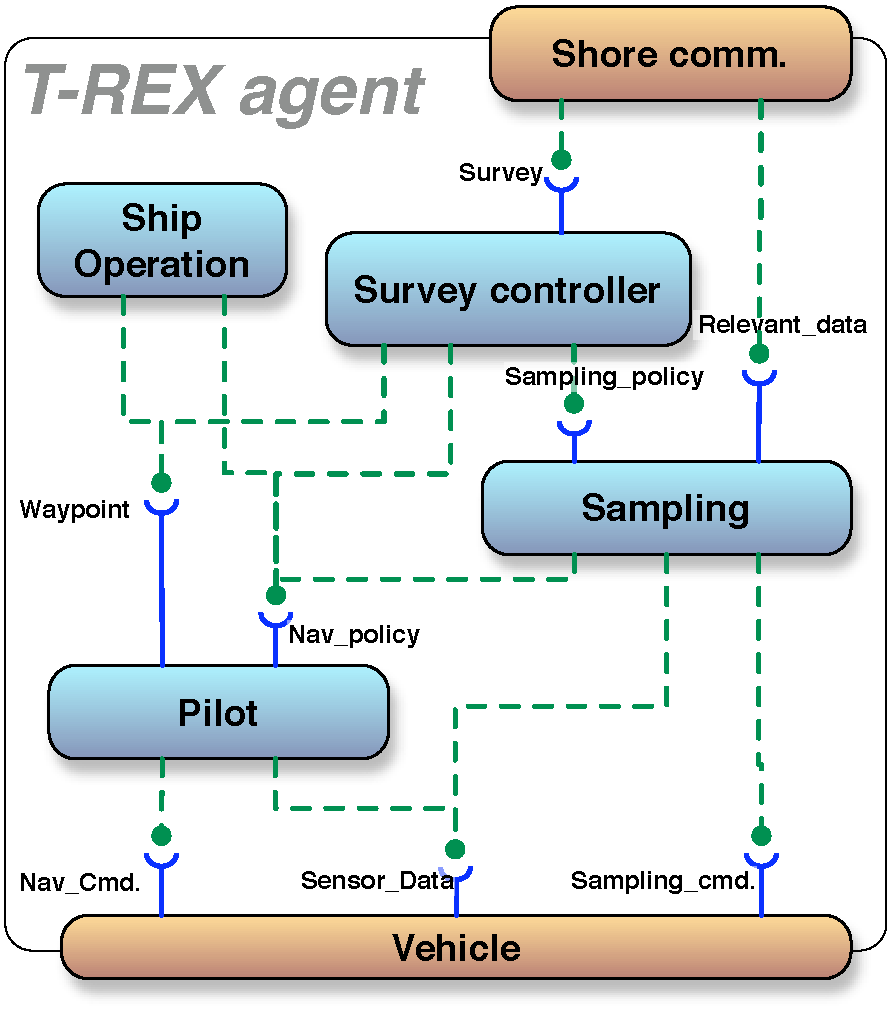
\includegraphics[scale=0.45]{figs/AUV-agent.pdf}
  \label{fig:agent}
  }
  \qquad
  \subfloat[\small State information flow between the
    \texttt{Pilot} and the \texttt{Vehicle} reactors.
    Observations transit as a bottom-up flow 
    and apply to the execution frontier $\tau$. 
    Goal information flow from the top to the bottom and relates to 
    desired future values of state variables.]{
      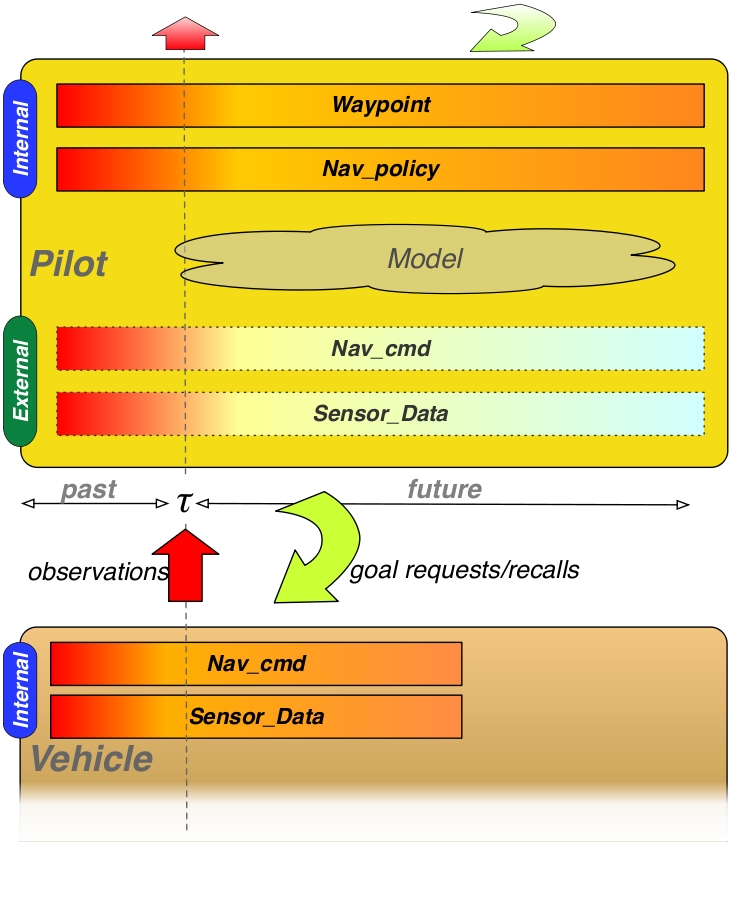
\includegraphics[width=0.4\columnwidth]{figs/TREX_flow}
      %\vskip-1cm
      \label{fig:trex:flow}
    }
    \caption{\rx connection of reactors through state variables based on the
    AUV agent we use at sea.}
\end{figure}

Consider for example the \rx agent instance we use on our AUV as shown
in Fig. \ref{fig:agent}. In this instance all the reactors (symbolized
by colored boxes) do not have an explicit connection from one to
another but instead rely on a publish/subscribe model on shared state
variables. For instance the \textsf{Pilot} reactor needs the {\em
  externally} managed state information from \textsf{Sensor\_Data} and
\textsf{Nav\_cmd} state variables in order to maintain the
\emph{internal} state variables \textsf{Waypoint} and
\textsf{Nav\_policy}. This relation applies in two ways:

\begin{itemize}

\item In order to identify its current {\em internal} state values the
  \textsf{Pilot} needs to know the current {\em external} state 
  information it relies on. This information is providede in turn by
  the reactors that provided these timelines as {\em internal}. In
  this specific case, the current \texttt{Waypoint} where the vehicle
  is heading can be evaluated based on the \texttt{Nav\_cmd} executed
  along with usefull \texttt{Sensor\_Data}, both being provided by the
  \texttt{Vehicle} reactor.

\item The future objectives a reactor has on \textsf{Internal} state
  will likely imply sub-objectives to be reported to the owner of its
  {\em external} state variables depending on their current
  values. Should the \textsf{Pilot} want to visit a specific
  \textsf{Waypoint} -- given its current position as provided by
  \textsf{Sensor\_Data}, it can identify a sequence of
  \textsf{Nav\_cmd} states that should eventually help it reach this
  location. %\comment{this explanation could do with a figure which I
    %believe we have used previously}

\end{itemize}

Given the above example, the \rx architecture therefore helps abstract
reactor interaction by constraining them to state variables. Each
reactor is therefore agnostic where its {\em external} state
information is managed as long as this information is available and
properly maintained for managing {\em internal} state
information. This {\em internal} state in turn may be used by other
reactors. Such a formalism also constrains reactor interaction to
state information exchange which comes in two forms as illustrated in
Figure \ref{fig:trex:flow}:

\begin{itemize}

\item {\em Observation on current state values}: This information
  propagates \emph{up} in the reactor dependency graph at the
  synchronization phase and occurs at the beginning of every
  tick. During this phase the agent provides updates to each reactor
  on their {\em external} state variables for this tick so as they
  could compute their {\em internal} state variable values for this
  same tick. By doing so we propagate a consistent view of that state
  of the world throughout all the reactors as time
  advances. %\comment{could do with a figure here}

\item {\em Goal request on future state}: This information propagates
  \emph{down} in the reactor dependency graph. In order to satisfy own
  {\em internal} objectives, a reactor may have a plan that relies on
  future values of one of its {\em external} state. When such a plan
  is identified the agent ensures that this part of the plan is given
  as a goal to the owner of the given {\em external} state
  variable(s). %\comment{could do with a figure here}

\end{itemize}

The choice of representation of state variables, observations and
goals is directly derived from \eu timelines and tokens.  While such a
rich representation allows exchange of state information in a formal
yet flexible manner, its translation into planning frameworks that
have an explicit representation of time (such as but not limited to
\eu) is often trivial.

\subsection{The Execution Cycle}
\label{sec:arch:exec}

The overall execution cycle of the agent is also abstracted out as a
continuous planning/deliberation cycle between all reactors. At the
agent interface level, each reactor provides only two abstract calls
that conceptualize execution:

\begin{itemize}

\item \texttt{synchronize} takes the last {\em external} observations
  as an argument and returns the {\em internal} observations for a
  reactor or a failure report.

\item \texttt{step} that accepts new goals requested (if any) on the
  {\em internal} timeline of a reactor and will execute one step of
  deliberation. In the context of \eu for example one deliberation
  step corresponds to a single flaw resolution (Section
  \ref{sec:europa:arch}) while ensuring that the resulting plan is not
  proven inconsistent. This implies that it also includes the
  backtracking of the search in such a case.  The returned value by
  the \texttt{step} function is a boolean which indicates whether the
  reactor needs an extra step to deliberate or if this last step
  resulted in a complete plan within the reactor's look-ahead. On the
  later, the part of the plan that concern this reactor {\em external}
  timelines is provided in order to be dispatched as goals to
  whichever reactor that is reponsible for these. \comment{By
    extending I may have saud things I developed below ... will have
    to check}
\end{itemize}

Both these deliberative functions have different scope and temporal
constraints. The \texttt{synchronize} call is considered as atomic and
will focus only on state inference for the current tick by identifying
the current value of {\em internal} state variables from the latest
updates on the {\em external} state variables. This process propagates
up in the reactor dependency graph at every tick to ensure that all
reactors are aware of the current state of the world. \texttt{step}
relates to a single decision step of the planning process which is
focused on the future evolution of state variables; it can take
multiple steps spanning multiple ticks for a reactor to produce a plan
that is both complete and valid. When such plan is identified
\comment{how? Is there a terminating condition? No more flaws but I
  washoping it would have been defined in \eu section} its {\em external}
timeline(s) are then dispatched to the corresponding reactors which
own these times and which in turn can start their own deliberation
\texttt{step}s to satisfy these new objectives. Consequently execution
occurs as these goals and plans propagate down in the reactor
hierarchy until they eventually become goals for the lowest level
reactor which -- instead of deliberating -- may just transform this
goal into a command for execution in hardware.

\begin{figure}[!htbp]
  \centering
  \vskip-1pc
  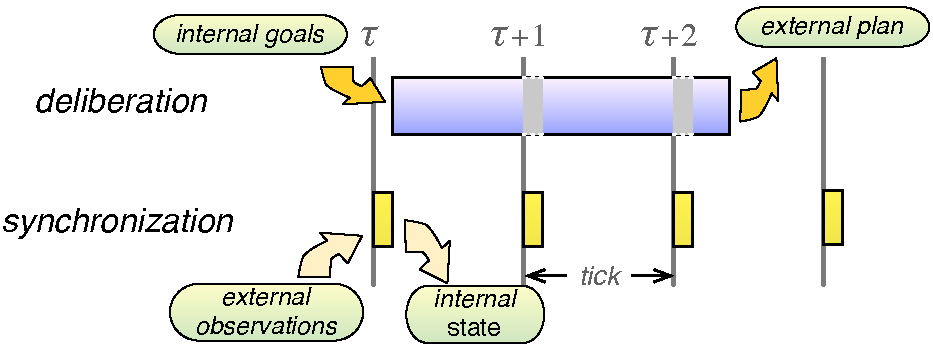
\includegraphics[width=0.55\columnwidth]{figs/tick-cycle}
  \caption{\small \rx reactor execution cycle: {\em Deliberation} is
    interrupted by {\em synchronization} at the beginning of every
    {\em tick} allowing integration of state information.}
  \label{fig:tick-exec}
  \vskip-0.8pc
\end{figure}

The manner in which the agent interleaves planning \texttt{step}s and
synchronization for a single reactor is illustrated in
Fig.~\ref{fig:tick-exec}. Synchronization occurs at every tick while
interrupting planning; this allows a reactor to identify its current
state that can propagate through the reactor hierarchy in order to
ensure a consistent view of the state of the world between all the
reactors.
% This view of a reactor has two parallel tasks allowing for long
% planning deliberation while ensuring that the state evolution
% propagates through the agent as time advance.
These intertwined tasks together provide two natural information flows
(bottom-up for state estimation and top-down for plan projection) that
we expect to see in a control loop. As they are both inference-based
processes it is natural to implement a reactor based on generic
automated planning. For example in Fig. \ref{fig:agent}, apart from
\textsf{Shore comm.} and \textsf{Vehicle} acting as interfaces to the
system, every other reactor (in blue) are different instances of a \eu
reactor differentiated only by their model and \eu solver
configurations.

\subsection{The  \eu Deliberative Reactor}
\label{sec:arch:europa}

Within \rx, an instance of an \eu reactor comes with the sole purpose
to deliberate. A typical design of such a reactor takes its cues from
\texttt{IDEA} \cite{mus02, mus06} where both planning and execution
are based on a single unified model within a rich representation that
provides support for temporal inference. In \rx, the execution cycle
consists of two deliberation processes which are implemented as two
\eu solvers modifying the \emph{same} plan database. %  and for which the
% execution is managed by the \rx framework as time advance during the
% execution of the system:

\begin{enumerate}

\item The \emph{synchronization solver} is a specialized \eu solver
  that integrates new information in the plan, the evolution of
  \emph{external} state variables and ensures that the reactor
  propagates these to identify the reactors current state as well as
  to inform other reactors of any state change on its \emph{internal}
  timelines. This solver is summoned at the beginning of every single
  tick.

\item The \emph{deliberation solver} manages the deliberation process
  of the reactor either to produce a new plan or alter its current
  plan as new goals are provided or when the synchronization solver
  identifies a conflict between current state and expectations from a
  previously generated plan. This process can span multiple ticks and
  can therefore be interrupted by the synchronization solver.

\end{enumerate}

While the two processes are separate, they share the same plan
internal to a reactor; consequently at every synchronization cycle the
planning process is informed of the new world state and its impact on
the plan. Conversely, when synchronization occurs after deliberation
steps, its starting point is the last partial plan resulting from
deliberation. This gives an initial frame to the problemm that helps
-- at least initial -- to target the synchronization problem by
ensuring that the new {\em external} state updates are compatible with
this plan. If so, the synchronization propagates these events in the
plan and can uses it as a help on identifying its {\em internal}
timelines based on this plan. If they are not compatibles, then
synchronization identifies a plan inconsistency  reflecting that the
current plan is not valid anymore. \comment{fpy: I am here and will
  develop further}

\comment{following is not what I intended to express whatsoever
  ... synchroniuzation od not deal with dispatching but execution
  tracking ... it is though helped by the structure of the exisiting
  plan and often identifies execution failures}
 Conversely, when the deliberation process eventually finds a
solution, synchronization is informed about generating the planned
state values \comment{should this read as ``...is informed about
  generated state values..'' instead?} on the {\em external} state
variables. This {\em external} plan defines the set of {\em goals} for
this state variable managed by another {\em reactor}.

Synchronization offers an important challenge for embedding planning
in a situated agent, typically %  as always been to go around the asumptions made by
% most classical planners. Specifically one
an assumption to restrict the problem to ``offline planning'' defined
in \cite{ghallab04} as follows:

\begin{quotation}
  The planner is not concerned with any change that may occur in
  $\Sigma$ \footnote{The world modeled by the plan domain.} while it is
  planning; it plans for the given initial and goal states regardless
  of the current dynamics, if any. 
\end{quotation}

This assumption, while helpful to reduce the scope of the planning
problem, becomes problematic for planning within a highly dynamic
environment. In a typical robot this implies that the only point where
the planner can be informed about the current world state is prior to
the commencement of a planning cycle by giving to the planner the
initial state and current objectives. During the planning, it is
assumed that the agent can maintin the world as perceived by the
planner as stable. \cite{lemai04, lemai-chenevier2004} attempts to
reduce the impact of planning by allowing local plan repair in the
existing plan. In the eventuality that such repair is not feasible
they require that their robot comes to a full stop until (re-)planning
is complete. \comment{I may need more examples/refs here}. As Fig.
\ref{fig:tick-exec} shows, this assumption is problematic for our
architecture. Synchronization that tracks state evolution can occur
several times during the reactor deliberation process. By making
synchronization and deliberation share the same plan we provide a
solution that relaxes this static world assumption. \comment{Need to
  talk about IDEA and the fact that they had similar aspect even
  though they were never very clear nor well articulated in their
  papers}

In the following sections we show how synchronization and deliberation
are implemented independently to show how their interaction through
the plan helps relax this assumption by making planning fully
integrated in the reactor execution cycle while potentially allowing
for more informed planning.

\subsubsection{Synchronization identify internal state evolution}
\label{sec:arch:synch}

We first show how a reactor can track and identify its state in the
context where it does not have any compelling need to deliberate. We
assume that we have a reactor that has no future goal. Even in this
condition, \rx requires each reactor to produce at every tick its {\em
  internal} state. For those reactors not owning {\em internal}
timelines, \rx makes sure that {\em external} observations are taken
into account for every tick as shown in \cite{py10}. Such a
requirement is enforced to ensure that all reactors share a consistent
view of the world with advancing time.

{\em External} state updates are managed by introducing these
observation in the plan structure as facts and ensure that they remain
compatible with the current plan mainainted by the reactor. The
challenging part of synchronization is to decide the {\em internal}
state values for the current tick. In the Shopping example for example
we have the following code snippet which helps identify when we can
\texttt{Buy} a product:

\begin{verbatim}
Agent::Buy {
  eq(duration, 10);
  // [...]
  contained_by(condition object.location.At currLocation);
  // [...]
}
\end{verbatim}

If \texttt{object.location} is {\em external} and the \texttt{Agent}
is {\em internal}, a robot may encounter the situation where it is at
the location where it can buy one (possibly among others)
product. This results om a decision problem related to the state value
of the \texttt{Agent} timeline where the robot can either {\em Buy} a
specific product now, wait a little longer before doing so or just
simply not buy any product at this location.

In the \eu based reactor this decision requirement is a new type of
flaw which forces full identification of internal state of the reactor
for the current tick. Using this new flaw we can describe the
synchronization process as:

\begin{enumerate}

\item Integrate the external state as provided by the owner of each
  external timeline into the plan database.

\item Propagate this information in the plan database following the
  model $\mathcal{M}$ of this reactor.

\item Resolve the current state value of each internal timelines.

\end{enumerate}

\begin{figure}[!htbp]
  \centering
  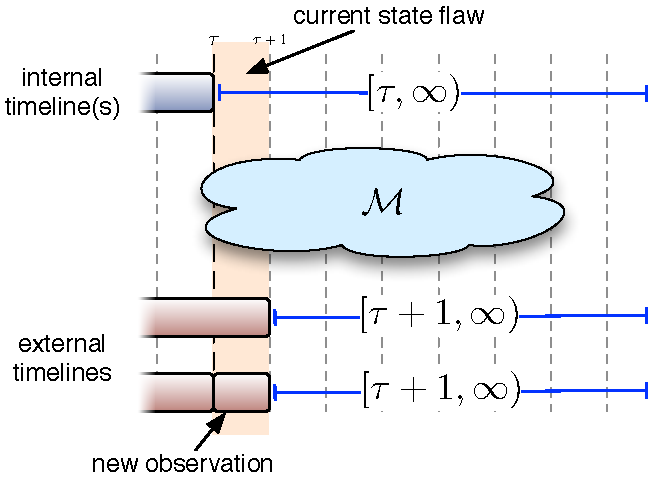
\includegraphics[width=0.5\columnwidth]{figs/synch-relation}
  \caption{\small Illustration of the synchronization flaws in a reactor. The
    reactor receive new observations when they are produced by the
    owner(s) of its internal timelines. The line after the last token
    of each timeline represent the domain of possible values for the
    end of this token. At every tick $\tau$ the reactor needs to
    integrate the {\em External} state information it received and --
    based on its model $\mathcal{M}$ -- resolve its {\em Internal}
    state that will then be provided by the architecture to other
    reactors using these state variables.}
  \label{fig:synch:flaw}
\end{figure}

We introduce this requirement as a new type of flaw for the \eu
framework defined as follow:

\begin{definition}
  \label{def:csf}
  A {\em current state flaw} indicates that a reactor {\em internal}
  timeline does not provide a fully defined state value for the
  execution frontier $\tau$. Such a flaw can be result of either of
  the following reasons:

  \begin{itemize}
  \item The absence of a token in this timeline which overlaps the
    instant $\tau$.
  \item An open decision between terminating the last token for this
    timeline or pushing its end in the future.
  \end{itemize}

\end{definition}

The core idea between this flaw is to ensure that at any single tick
the {\em synchronization} solver will identify all the {\em internal}
timelines for which the current state value is yet to be
identified. We handle their resolution based on the following
proposition.

\begin{proposition}
  \label{prop:csf:resolve}
  A {\em current state flaw} can be resolved using one of the
  following choices which are evaluated in the following order:

  \begin{enumerate}

  \item Extend the previous state value to end after the execution 
    frontier  (\ie restrict its end time to $[\tau+1, \infty)$). %\comment{first use of
    % $\tau$, so needs to be defined earlier}

  \item Start the next active token in the timeline by restricting its
    start time to the single value $\tau$

  \item Create and insert a new token in this timeline that will start
    at the current tick $\tau$ (attempt this for each possible token
    type for this timeline if necessary).

\end{enumerate}
\end{proposition}
Intuitively the first choice enforces an intertial value assumption
where the reactor will tend to maintain its current as long as the
model and external observations allow it. The second choice favorise
the advance of the reactor current plan if any; this direct the {\em
  synchronization} decision toward assuming that its current plan is
properly executed. Finally if none of these two choices did provide a
valid solution -- meaning that both lead to an inconsistant plan --
the reactor tries all the possible state values remaining for this
timeline until it finds one that allows it to identify its state as
required by \rx architecture.

This flaw forces the reactor to identify its internal state
for the current tick. By using this flaw one can describe the
synchronization process as:

\begin{enumerate}
\item Integrate the external state as provided by the owner of each
  external timeline into the plan database.
\item Propagate this information in the plan database following the
  model $\mathcal{M}$ of this reactor.
\item Resolve the current state value of each internal timelines based
  on Proposition \ref{prop:csf:resolve}.
\end{enumerate}

%%%% Extra paragraph:  targeted to a more AI centric audience
% The step 1 translates new {\em external} observations received from
% \rx into europa tokens with a start time restricted to $\tau$ or, for
% the timelines that did not receive a new observation,  restrict the
% previous token end time to the interval $[\tau+1, \infty)$. All of
% these tokens are produced as facts and consequently cannot be 
% excluded from the plan. They are also maintained by the reactors as
% observation tokens which will allow to avoid to mistakenly remove 
% them when one of the two reactor solvers attempt to relax former
% decisions made.\comment{This relaxation is developed on the last 
%   subsection further in depth}
%%%%

Steps $2$ \& $3$ are handled by the \eu solver from algorithm
\ref{alg:europa:solve}. We only enforce that the {\em current state
  flaws} are selected last by the algorithm in order to follow the
sequencing given above. As {\em synchronization} focusses on the
execution frontier wee also filter out all flaws that are outside of
the current tick scope. This mean that if this flaw relates to a token
that is {\em necessarily} ending before $\tau$ or starting after
$\tau+1$ then the solver will ignore it. This helps to reduce the
scope of the synchronization to exclusively the current state of the
reactor and reduce dramatically the search space for the {\em
  synchronization} solver. In order to do so we need to assume 
that the current state value of an {\em internal} timeline does not 
depend on the future or more accurately that any choices made during 
this {\em synchronization} will not lead to a future inconsistency. 
Such an assumption impacts the set of possible domains the reactor 
can support while remaining complete. Take for  example this rule from 
our \texttt{Shopping} model :

\begin{verbatim}
 1 Agent::Go {
 2   met_by(condition object.location.At origin);
 3   eq(from, origin.loc);
 4
 5   equals(effect object.location.Going going);
 6   eq(going.from, from);
 7   eq(going.to, to);
 8   
 9   meets(effect object.location.At destination);
10   eq(to, destination.loc);
11 }
\end{verbatim}

While this model is perfectly acceptable for planning it becomes
problematic when execution is taken into account especially since it
puts a strong emphasis between an evolving plan and an unknown future
(\texttt{Going} to a location and the {\em expected} future outcome of
ending at this location, ties it strongly to the constraint in line
$5$ above).  So for example, assume that the \texttt{Agent.location}
is {\em external} to the reactor which receives the observation
\texttt{Going(Home,SuperMarket)} which synchronization has resolved by
producing the observation \texttt{Go(Home, SuperMarket)} in the
\texttt{Agent} timeline. This would imply that the only possible
outcome on \texttt{Agent.location} is to be \texttt{At(SuperMarket)}
in the directly foreseeable future. In the real world the fact that we
are \texttt{Going} to a certain location does not necessarly imply
that we will succeed on ending up there. In one extreme case due to an
exogenous event, the road to the \texttt{SuperMarket} is closed which
could result in an alternate observation that the robot is
\texttt{At(7th st. \& Main)}. This observation contradicts the
existing plan the reactor is maintaining. Further, it is important to
understand the temporal direction of the \emph{causal link} that is
triggering the inconsistency. At the time the robot observes this
contradicting the \texttt{At} predicate, the rule that generated this
conflict is connected to past observations \texttt{Going} and
\texttt{Go} which cannot be easily retracted without a potential
global impact to the plan implying a huge cost in back-propagation
that would be problematic.

More generally tying a token to future outcomes in a model that is
meant to be confronted by execution is problematic. It might be valid
if one can guarantee that an outcome is predisposed to occur (for
example the reactor managing \texttt{Agent.location} timeline
guarantees that the outcome of the \texttt{Going} will {\em always}
result on ending at the traget location). However, given the very
nature of the planning problem and the ability to search outcomes and
replan, the model should be written so that a future projection can be
manipulated. %  while keeping in mind that predicting the future is not
% absolute. 
In this case one could alter this part of the model in order to give
the reactor more flexibility as follows:

% \begin{minipage}[t]{\textwidth}
% \begin{figure}
\begin{verbatim}
 1 Agent::Go {
 2   met_by(condition object.location.At origin);
 3   eq(from, origin.loc);
 4
 5   contains(effect object.location.Going going);
 6   eq(going.from, from);
 7   eq(going.to, to);
 8   
 9   meets(effect object.location.At destination);
10   eq(to, destination.loc);
11   going meets destination;
12 }
\end{verbatim}
% \label{lab:model:shopping}
% \caption{\small Model fragment to enforce a \texttt{Going} end condition}
% \end{figure}
% \end{minipage}

We do so by relaxing the constraint in line $5$ from a strict
\texttt{equals} to a \texttt{contains} and to add the new constraint
at line $11$ which ensures that the last \texttt{Going} ends up in the
location the agent actually wants to be at. This first level of
relaxation will therefore allow the agent to use multiple
\texttt{Going} tokens should the first one fail to reach the
objective.  % The problem can even be relaxed further if needed but
% this relaxation gives already more flexibility for the reactor to
% recover from local failures.
As the simple example above shows, synchronization involves a
deliberation process with the risk that the search for a solution is
not a straightforward sequence of unit decisions. Since such a process
is required by the architecture at \emph{every} tick for \emph{every}
reactor the model needs to be carefully designed.

One critical aspect to take into account is that from a \rx point of
view, synchronization is the only critical task of a reactor. Such a
process is used in order for the agent to identify its current state
and maintain it consistently throughout the agent's lifetime. For a
reactor not being able to find a consistent solution during
synchronization -- implying that after evaluating all possible
solutions provided by a model it was unable to find a consistent plan
-- not only indicates that a reactor is unable to explain the state of
the world, but more importantly it may jeopardize other reactors that
rely on its {\em internal} state. For this reason a failure to
synchronize immediately results in the agent killing a reactor and
notifying any reactor that depends on its {\em internal} state
variables; it does so by posting the special observation
\textsf{Failed}. And by doing so we allow for graceful degradation
where other reactors can readapt their plans as they receive this
observation.

Finally, at the engine level careful choices were made in 
both the focus of the search -- limited only to tokens that 
can potentially overlap the current tick -- and heuristics where 
the {\em current state flaw} is considered last during the search
process. The later limits the amount of backtracking for a solution 
-- or at least how deep one needs to backtrack in a decision tree. 
Similarly the sequence in which we evaluate the possible resolution 
for such a flaw -- presented in Proposition \ref{prop:csf:resolve} -- 
was selected according to  some simple assumptions that any external 
observation that is compatible with an existing token in the current
plan reflects the execution of the plan itself. In other words this
means that our solver always prefer to use tokens already existing in
the plan in order to identify its current internal state. By doing so
we directs the synchronization search by exploiting the structure of
the plan produced during previous deliberation steps. This implies
that a deliberation steps have been done and did impact the plan
structure and calls for a description on how our \eu reactor resolve
such steps which we are now going to describe further.

\subsubsection{Deliberation: Planning for future state evolution}
\label{sec:arch:plan}

Deliberation inside a reactor is based on \eu capabilities described
in Section \ref{sec:europa:arch}. However deliberation within \rx
comes with some augmentation -- deliberation information one reactor
provide to the architecture such as its deliberation latency and its
plan look-ahead both expressed in ticks -- and the fact that we
potentially need to interleave deliberation with not just the
synchronization process but also with deliberation of other
reactors\footnote{The current implementation of \rx is running on a
  single process and it is the responsibility of the agent itself to
  emulate reactor multi-threading for deliberation and
  synchronization.}. For this reason while the overall planning of a
deliberative reactor strictly relies on the \eu framework planning
solver, it slices the execution of Algorithm \ref{alg:europa:solve} in
atomic steps. The interruption is done around the recursive call (line
\ref{li:recurse}) while ensuring that the current partial plan is
never proven inconsistant at any single step. This can be managed by
allowing the call to backtrack until a \textsf{DecisionPoInt} that is
not exhausted (\ie $decision.hasNext()$ is \texttt{true}) is found in
the call stack.

A critical aspect of this deliberation step is to ensure that at the
exit of this call the $plan$ is not inconsistent. % Indeed, it is always
% possible that the next call made by the agent is for synchronization
% which could fail if the $plan$ is inconsistent before any attempt is
% made for synchronization.
If the partial plan is found to be inconsistent during a deliberation
step we either backtrack in the decision stack until a node of the
tree is found with an alternate solution or the plan is relaxed since
there is no other alternative solution. We do this by removing all
goals and keeping only recent observations. % These constraints are yet
% again related to the fact that for the agent the only crucial
% functionality of a reactor is to resolve successfully its
% synchronization.

The number of flaws between two steps \comment{between synch. and
  execution?} can evolve for the following reasons that are exogenous
to deliberation:

\begin{enumerate}

\item A new goal has been posted on a reactor timeline. This is
  usually due to another reactor finding a partial plan and posting
  the corresponding new objective.

\item The outcome of synchronization created new flaws that did not
  need to be resolved during synchronization.

\item A previously requested goal has be recalled by the initial
  requester. This can occur when the reactor's initial plan is no
  longer valid, for instance with synchronization resulting in
  inconsistency.

\end{enumerate}

\comment{this might be a subsubsection before someplace since it
  introduces the concept of latency/lookahead.}
These events could potentially produce new flaws to be resolved while
any single deliberation step will likely reduce the number of flaws
for resolution. The scope of planning for a reactor also plays a role
in the deliberation process as we limit deliberation to the sliding
temporal window $[\tau+\lambda, \tau+\lambda+\pi]$ \cite{py10} where:

\begin{itemize}

\item $\tau$ is the current tick indicative of the execution frontier 

\item $\lambda$ is the specified latency of this reactor, which is an
  indicator of the maximum expected time for a reactor to produce a
  plan.\footnote{Note that while it is highly recommended to select a
    sound value, a failure to produce a plan within a chosen value for
    this parameter is not considered as a critical failure of the
    reactor.}

\item $\pi$ is the planning look-ahead of the reactor. which indicates
  how many ticks in the future this reactor is looking ahead during
  deliberation. 

\end{itemize}

\comment{Insert a figure here [AAMAS?] showing $\pi \lambda$} Such a
scope allows filtering of tokens that are either necessarily ending
before $\tau$ or necessarily starting after, focusing the planning
problem on only those tokens that are within a ``reasonable''
future. This window is taken into account by the \rx agent which will
notify a reactor of new {\em internal} goals not only when they
overlap this reactor specific window but also for the deliberation
solver in order to reduce the number of tokens to be evaluated to
reduce deliberation cost and performance. As time advances flaws that
were initially beyond this temporal horizon will become active which a
reactor can evaluate. This results in an apparent \emph{continuous
  planning} of the reactor. When there are no more flaws present in
the current planning scope a partial plan solution is found. This has
two effects:

\begin{enumerate}

\item This reactor does not need to deliberate until the next
  synchronization. 

\item The token on the {\em external} timelines of this partial plan
  can then be posted which eventually (at the end of the current tick
  if these goals overlap the owner reactor's planning window) will be
  dispatched as goals, in turn triggering further deliberation.

\end{enumerate}

\subsubsection{Intertwining synchronization and execution}
\label{sec:arch:intertwine}

One key aspect of the \rx framework is intertwined plan execution. As
seen above, it is synchronization which drives planning, so the
co-mingling between these two processes is critical to maintaining
state within a robot immersed in a dynamic environment. Also important
is that \rx maintains 
% A core aspect of this reactor is that it takes advantage of the
% specific sequencing enforced by the \rx architecture along with the
% fact that only 
one $plan$ structure in the reactor and shared between synchronization
and planning. This allows these two processes to not only be
interleaved but how they can impact each other via plan manipulation.

The most obvious case is how synchronization allow propagate of {\em
  external} observations as a new tick occurs. In our presentation of 
{\em synchronization}, we isolated the problem by stating
that we will assume at this point that the reactor has no future goal
or more accurately no plan to enforce. By doing so we
were able to develop the way we augment the \eu solver to be able
to propagate {\em external} observations in order to identify the
reactor {\em internal} state for the same tick. This allowed us 
to focus on synchronization as a state evaluation process that can
be resolved within the \eu framework with few extensions. Similarly
we presented deliberation at this fairly high level not necessarily
discussing how the disruptive nature of synchronization in this
process could impact the way this planning could evolve.

We first analyze the case during which synchronization occurs after
planning has completed (\ie the last step of deliberation results in a
plan that is considered complete for the current look-ahead). As
synchronization starts with a plan % produced this will gave a frame for
% the search process. Therefore 
this deliberation will not only be a model-derived estimation uniquely
based on {\em external} observations but will also include reactor
intentions specified in the available partial plan. Consider for
example the Shopping Agent model described where the \texttt{Agent} is
an {\em external} timeline. As the reactor adds the goal to
\texttt{Own} milk and the current {\em external} timeline indicates
that the robot was \texttt{At(home)}, it produces a plan as shown in
Fig. \ref{fig:shop:exec0}. The {\em external} part of the plan --
namely the tokens \texttt{Going(home, superMarket)} and
\texttt{At(SuperMarket)} -- are installed as goals for the reactor
managing this state variable {\em internally}.

\begin{figure}[!htb]
  \centering
  \subfloat[\small A plan produced before synchronization.]{\label{fig:shop:exec0}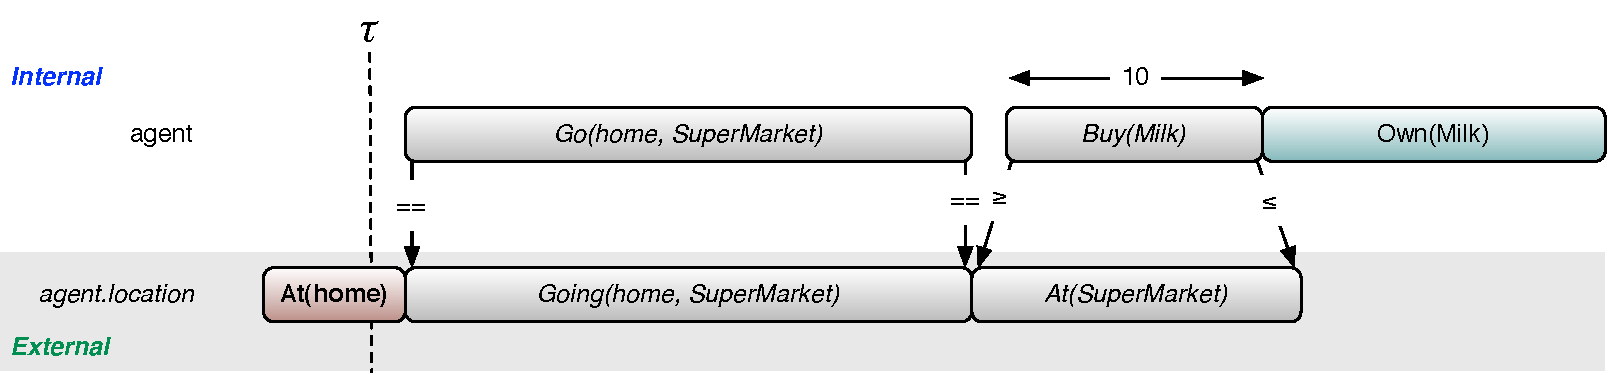
\includegraphics[width=0.45\columnwidth]{figs/shoping_exec_t0}}
  \subfloat[\small Result of synchronization after the {\em Going}
  observation was received by the reactor with the plan showed in
    \ref{fig:shop:exec0}.]{\label{fig:shop:exec1}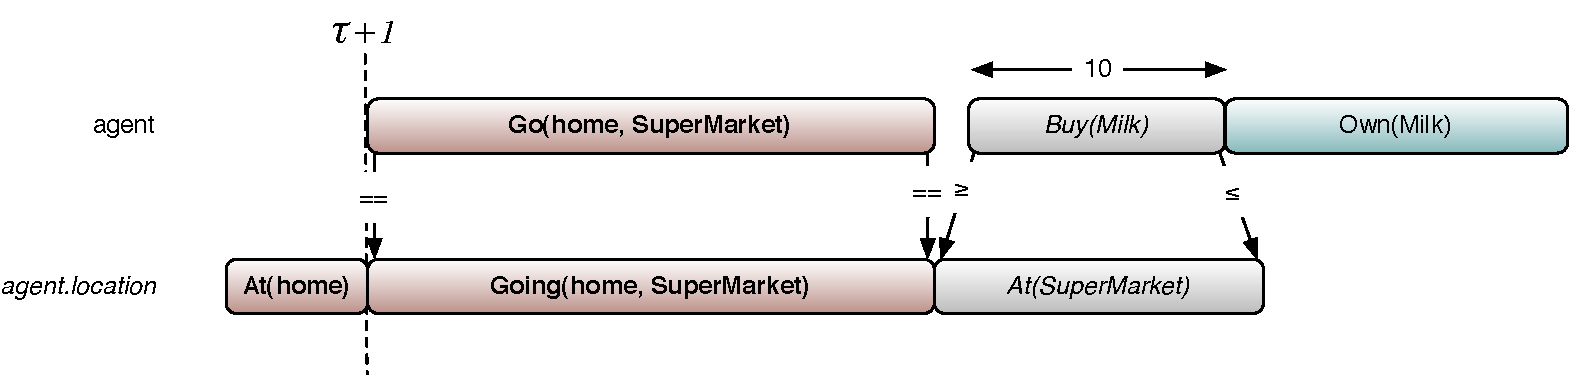
\includegraphics[width=0.48\columnwidth]{figs/shoping_exec_t1}}
    \caption{\small Shopping example: Tokens in red indicate
      observations, tokens in blue the goal that this plan attempts to
      solve for. Arrows indicate temporal constraints. }
  \label{fig:shop:exec}
\end{figure}

Consider that at the next tick $\tau' = \tau+1$ the reactor managing
agent location is able to change the location state variable to
\texttt{Going}. \rx informs our reactor of this new observation which
is added in the plan structure as a fact -- starting exactly at
$\tau'$ and lasting for an unknown duration which is at least 1
tick. As this new observation is integrated in the plan through
synchronization, the solver can identify the similarity between this
observation and the next token in the existing plan. Instead of
initiating an exhaustive search of all possible implications, the
synchronization process starts its execution with the assumption that
these new observations are consistent with the currently maintained
plan. As a consequence, at the end of synchronization the plan
depicted in Fig. \ref{fig:shop:exec1} is likely. This is a result of
propagation of information provided by the new observation in the
existing plan while restricting the start time of \texttt{Going} and
propagating temporal constraints, making \texttt{Go} to start {\em
  exactly} at $\tau'$. In doing so, the \eu solver's focus on the
execution frontier ($\tau'$ in Fig. \ref{fig:shop:exec1}) takes
advantage of the existing plan to evaluate a solution that assumes
that the observation is consistent with what was decided by the
reactor.

% \begin{figure}[!htb]
%   \centering
%   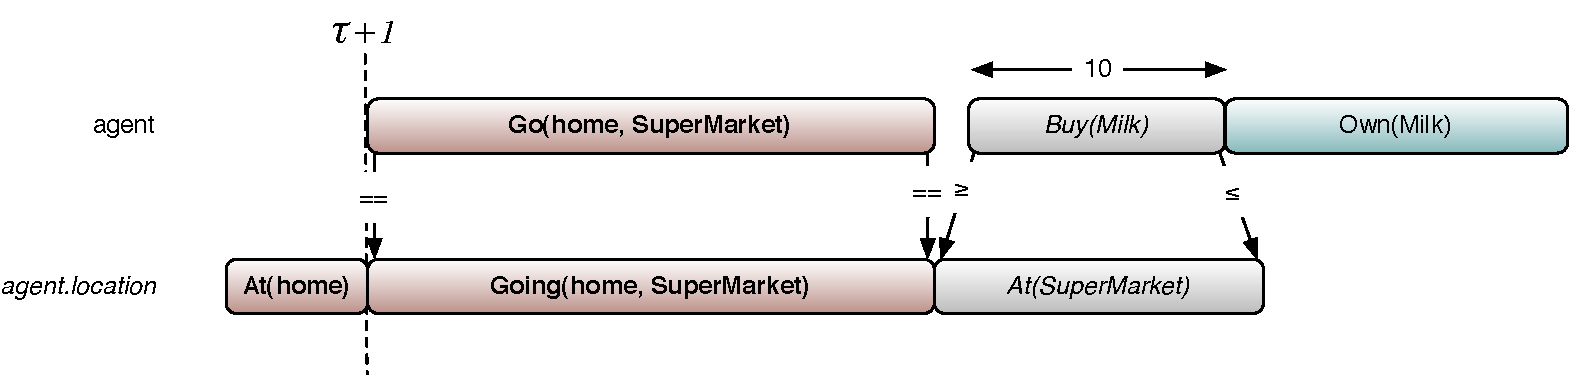
\includegraphics[width=0.7\columnwidth]{figs/shoping_exec_t1}
%   \caption{Shopping example : Result of synchronization after the {\em
%       Going} observation was received by the reactor with the plan
%     showed in Fig. \ref{fig:shop:exec0}.}
%   \label{fig:shop:exec1}
% \end{figure}

This choice is directed not only by heuristic choices made in the
solver but also enforced by the heuristic order of the decision point
resolution choices for the {\em current  state flaw} presented in
Proposition \ref{prop:csf:resolve}. Indeed, as we stated then the two
first choices tend to privilege a conservative view in respect to the
existing plan. It attempts first to extend the previous observation we
produced for this {\em internal} timeline in order to avoid to commit
to early in the plan advance. If the formaer failed it will then
attempt to start the next exisiting token in the plan which alow the
reactor to advance its plan execution. Both of these two initial
choices atetempt to resolve the plan with the least amount of
perturbation of the plan. They just constrain further the start and
end time of the exisiting tokens which were provided by the previous 
deliberations steps. This means that in a nominal situation where the
plan this reactor produced is properly executed, the synchronization
remains limited to restrict time points in the plan and progate their
impact. Most of the heavy dutty work of creating new tokens in the
plan and schedule them -- both being much more difficult problems 
to resolve -- have been managed during deliberation steps. In that
sense we see that most of the time synchronization is limited to very
few node in \eu search space with often no backtrack required. The
synchronization may become slightly nore costfull when we need to
identify a new token to be injected by the plan (the 3rd choice in
Proposition \ref{prop:csf:resolve}) as it needs to explore on tis own
all the possible token types this timeline accept as value. This is
the reason this choice is evaluated last in our flaw resolution in
order to avoid such complex action during synchronization unless 
necessary. In that sense,  ansd due to carefull choice on our
synchrponization heurisitic we see that the plan produced during \rx
deliberation steps helps sthe synchronization process to be more
efficient. 

% Should such a flaw be revealed 
% during synchronization -- such that the current state of
% an {\em internal} state variable is not fully grounded -- the
% sequencing of the choices will attempt first a conservative choice in
% maintaining previous state and only then try a more optimistic
% approach in terms of the \comment{I don't follow this last bit. Is
%   this token addition that you're talking about?} execution/advance in
% our current plan to finally attempt other choices that were not
% predicted by the model. The two first possible choices are strongly
% directed by the existing plan which helps direct the search within
% this frame. This often allow to have a synchronization that is much
% more directed and, in nominal cases such as the one we showed resolve
% the deliberation in few steps (often without any backtrack in the
% search) \comment{All this is confusing; probably reword}.

Synchronization also supports the tracking of plan execution. It does
so by specifying token parameters such as time points that are
propagated through the plan in order to identify if the plan remains
valid -- as in our example -- or that it cannot be executed as it
is. The later is often identified by the synchronization failing to
find a consistent solution. For example should the \texttt{Going}
observation received be to the \texttt{hardwareStore}, this would
break the current partial plan in the reactor as the robot cannot
possible be going simultaneously to $2$ different locations; see
Fig. \ref{fig:shop:relax1}. As synchronization is not possible in such
a situation the strategy followed is to relax all decisions made by
previous plan steps. This is done by keeping all past observations in
both {\em external} and {\em internal} state variables as well as the
existing {\em internal} goals (\texttt{Own(Milk)} in this example)
received by this reactor. The resulting partial plan is shown in
Fig. \ref{fig:shop:relax2}. In this process the reactor informs the
agent that all {\em external} goals it requested for the future are no
longer valid which results in turn, in timeline owners not having to
maintain such goals.

\begin{figure}[!htbp]
  \centering
  \subfloat[Conflicting Observation]{\label{fig:shop:relax1}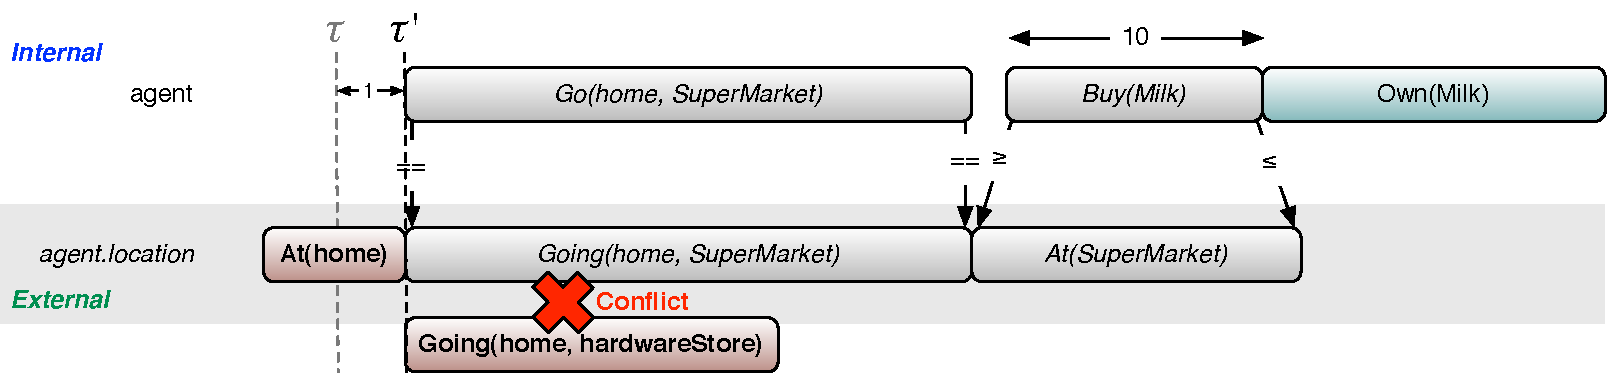
\includegraphics[width=0.7\columnwidth]{figs/shoping_exec_relax-1}}\\
  \subfloat[Relaxed Partial Plan]{\label{fig:shop:relax2}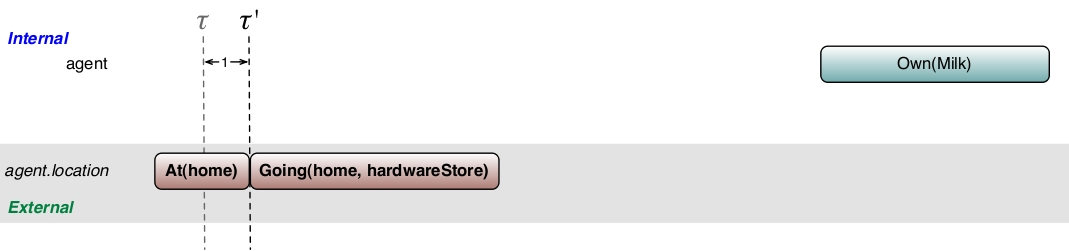
\includegraphics[width=0.7\columnwidth]{figs/shoping_exec_relax-2}}
  \caption{\small Illustration of a conflict during synchronization
    and the resulting relaxed plan for recovery.}
\end{figure}

As the plan is no longer conflicted, synchronization can resume and
find a solution described above. Newly pending goals would be enforced
at the next \texttt{step} to resume deliberation on this relaxed
partial plan. By using synchronization the reactor was not only able
to identify that its plan was not consistent but able to recover from
it by offering a new incomplete partial plan to be resolved in the
next deliberation \texttt{steps}. % This on its own offer the core
% functionality one should except to close the loop between planning and
% execution in the sense that 
Synchronization plays the role of what is typically termed as the {\em
  Executive} in other architectures \cite{gat98, alami:1998p820,
  mus98, williams03, Nesnas:2003do}.

In \rx however the interaction between planning and execution does not
stop at this level. The overall scheduling of both {\em
  synchronization} and {\em planning} is such that the synchronization
can occur in between any planning step. Not only is synchronization
influenced by the outcome, but it also influences
planning. Specifically when synchronization occurs before a complete
plan is found, it will inject new facts ({\em external} observations
and resulting {\em internal} state) in the plan database available for
inference when the next planning \texttt{step} resumes. On this next
step the \eu solver used for planning will have these new facts
included in the partial plan which can introduce new flaws in the plan
while potetnially having reolved previously exisiting flaw. The
deliberation process is therefore perturbed externally by the {\em
  synchronization} and consequently fully informed of the world state
evolution as it is planning.  This specific aspect contrasts with
other more classical approaches we have seen, which avoid 
perturbing the planner during its search as it is not compatible 
with the ``off-line planning'' assumption.

By our design choices -- both at the architecture level and the
integration of the \eu framework for embedded deliberation -- we are
able to implement an architecture that avoids this critical off-line
planning limitation while remaining within a formal framework that
allows for deliberation and model-based agent control. We believe that
this tight integration of planning and execution allows the system to
be more acute vis-a-vis the environment allowing informed
decision-making and a tighter reaction loop. This is possible while
integrating information despite a long latency for the reactors, as
long as one can ensure that synchronization of all reactors and
deliberation steps can be done within a time that is resonably small
in comparison to the agent tick duration.





% Gives a high-level overview of T-REX, the general design principles and how
% these principles aid in software engineering. Show T-REX block diagram.



%%% Local Variables: 
%%% mode: latex
%%% TeX-master: "setobook"
%%% End: 
